\documentclass[12pt,a4paper]{report}

%% Language and font encodings
\usepackage[french]{babel}
\usepackage[utf8]{inputenc}
\usepackage[T1]{fontenc}


%% Sets page size and margins
\usepackage[a4paper,left=2cm,right=2cm,top=2cm,bottom=2cm]{geometry}
\usepackage{titlesec}
\usepackage{listings}
\usepackage{hyperref}
\usepackage{graphicx}
\usepackage{tabularx}
\usepackage{float}
\usepackage{xcolor}

\lstset{language=C}

\title{Projet de fin d'étude \\ Chiffrement de disque LUKS sous FreeBSD}
\author{Romain CHERRÉ, Pierre KOEBELIN}

\titleformat{\chapter}[block]
  {\normalfont\huge\bfseries}{\thechapter.}{1em}{\Huge}
\titlespacing*{\chapter}{0pt}{-19pt}{0pt}

%\renewcommand{\thechapter}{\arabic{chapter}}
%\renewcommand{\thesubsection}{\thesection. \arabic{subsection}}
%\renewcommand{\thesubsubsection}{\thesubsection. \arabic{subsubsection}}

\lstset{literate=
  {á}{{\'a}}1 {é}{{\'e}}1 {í}{{\'i}}1 {ó}{{\'o}}1 {ú}{{\'u}}1
  {Á}{{\'A}}1 {É}{{\'E}}1 {Í}{{\'I}}1 {Ó}{{\'O}}1 {Ú}{{\'U}}1
  {à}{{\`a}}1 {è}{{\`e}}1 {ì}{{\`i}}1 {ò}{{\`o}}1 {ù}{{\`u}}1
  {À}{{\`A}}1 {È}{{\'E}}1 {Ì}{{\`I}}1 {Ò}{{\`O}}1 {Ù}{{\`U}}1
  {ä}{{\"a}}1 {ë}{{\"e}}1 {ï}{{\"i}}1 {ö}{{\"o}}1 {ü}{{\"u}}1
  {Ä}{{\"A}}1 {Ë}{{\"E}}1 {Ï}{{\"I}}1 {Ö}{{\"O}}1 {Ü}{{\"U}}1
  {â}{{\^a}}1 {ê}{{\^e}}1 {î}{{\^i}}1 {ô}{{\^o}}1 {û}{{\^u}}1
  {Â}{{\^A}}1 {Ê}{{\^E}}1 {Î}{{\^I}}1 {Ô}{{\^O}}1 {Û}{{\^U}}1
  {œ}{{\oe}}1 {Œ}{{\OE}}1 {æ}{{\ae}}1 {Æ}{{\AE}}1 {ß}{{\ss}}1
  {ű}{{\H{u}}}1 {Ű}{{\H{U}}}1 {ő}{{\H{o}}}1 {Ő}{{\H{O}}}1
  {ç}{{\c c}}1 {Ç}{{\c C}}1 {ø}{{\o}}1 {å}{{\r a}}1 {Å}{{\r A}}1
  {€}{{\euro}}1 {£}{{\pounds}}1 {«}{{\guillemotleft}}1
  {»}{{\guillemotright}}1 {ñ}{{\~n}}1 {Ñ}{{\~N}}1 {¿}{{?`}}1
}
\lstdefinelanguage{bash}{
  basicstyle=\normalfont\ttfamily,
  showstringspaces=false,
  breaklines=true,
  frame=single,
  backgroundcolor=\color[HTML]{EEEEEE},
}

\begin{document}
\maketitle

\tableofcontents
\newpage

% Chapitre 1: État de l'art
\chapter{Etat de l'art}

\paragraph{}
Ce projet consiste en la réalisation d'un module noyau pour FreeBSD rendant
possible l'utilisation d'un volume chiffré avec
\textit{LUKS}\cite{onDiskFormatLuks}, un standard de chiffrement associé au
noyau Linux.
\paragraph{}
L'objectif est donc de relever et comparer les moyens de chiffrement de disques
actuels, et d'analyser plus particulièrement les modules noyau Linux et FreeBSD
gérant le chiffrement de volume afin de porter le standard
\textit{LUKS}\cite{onDiskFormatLuks} vers FreeBSD.

\section{Différents niveaux de chiffrements}

\subsection{Chiffrement à la volée}
\paragraph{}
Le chiffrement de disque est généralement géré par le noyau du système, ou par
des logiciels spécialisés comme TrueCrypt ou VeraCrypt sur Windows. Il permet de
chiffrer et déchiffrer des partitions entières à la volée. Le disque, une fois
déchiffré, peut-être montré comme n'importe quel autre espace de stockage. Son
utilisation est totalement transparente pour l'utilisateur.
\paragraph{}
Dans des systèmes comme Linux ou FreeBSD, le chiffrement et déchiffrement du
disque est réalisé directement par le noyau. Au moment de la lecture et de
l'écriture du disque, les données passent par une couche supplémentaire
(\textit{dm-crypt} pour Linux et \textit{GELI}\cite{manGeli} pour FreeBSD) dont
le rôle est de faire le lien entre les données chiffrées du disque et celle en
claire visibles et utilisables par l'utilisateur.
\paragraph{}
Le fait que la lecture d'un disque soit faite par le noyau permet à un système
utilisant cette méthode de chiffrer tout le système, à l'exception d'une petite
partie permettant de déchiffrer le noyau au démarrage. Le reste du système peut
ensuite être directement déchiffré par le noyau.

\subsection{Chiffrement au niveau du système de fichiers}
\paragraph{}
Le chiffrement de système de fichier consiste en la création d'un système de
fichier qui sera ensuite enregistré chiffré sur le disque. C'est nottament la
technoligie utilisée par l'\textit{Encrypting File System} (abrégé EFS), une
technologie Microsoft disponible dès la troisième version des systèmes de
fichiers NTFS. D'autres solutions existent également, comme EncFS. Des logiciels
comme TrueCrypt/VeraCrypt permettent également de réaliser de genre
d'opérations, en chiffrant des fichiers dans un conteneur.
\paragraph{}
Le type de chiffrement a l'avantage de chiffrer toute une arborescence de
fichiers indépendamment des autres fichiers présents sur le disque. Cela permet
d'avoir différentes clés de chiffrement par système de fichiers chiffrés,
contrairement au chiffrement de disque qui en impose une seule par partition.
\paragraph{}
Ce type de chiffrement peut cohabiter sur un système utilisant déjà le
chiffrement de disque. Il ne permet en revanche pas de chiffrer des fichiers
nécessaires au démarrage du système, contrairement à l'autre type de
chiffrement.

\subsection{Chiffrement de fichier}
\paragraph{}
Ce type de chiffrement permet de chiffrer un seul fichier. Il peut s'agir
d'archives possédant cette propriété de pouvoir être chiffrées et déchiffrées
par les logiciels spécialisés. Dans ce cas, seul le contenu de l'archive est
chiffré et les métadonnées restent en clair. C'est le type de chiffrement
utilisé par des archives comme \textit{7z}. Le chiffrement peut également se
faire directement sur un fichier, en utilisant des solutions comme
\textit{gpg}, en créant un nouveau fichier \textit{.gpg} étant le chiffré de
celui d'origine.

\subsection{Chiffrement matériel}
\paragraph{}
Le chiffrement matériel (\textit{Hardware-based full disk encryption},
\textit{FDE}) concerne certains disques (appelés \textit{Self-encrypting drive})
ou autres espaces de stockage. Leur fonctionnement est basé sur le contrôleur
qui gère les clés de chiffrement servant au chiffrement du disque, et
œuvrant indépendamment du processeur. L'authentification se fait alors avec un
via un logiciel s'exécutant avant le démarrage du système ou mot de passe dans
le BIOS.
\paragraph{}
Le groupe \textbf{Trusted Computing Group} réunissant plusieurs fabricant a mis
en place une spécification, \textit{Opal Storage Specification}, pour ce type de
disques auto-chiffrés.

\section{Chiffrement de disque sur Linux et FreeBSD}
\paragraph{}
Le chiffrement de disque sous Linux et FreeBSD est géré par des modules noyaux
qui interviennent au moment de la lecture et l'écriture du disque. Les
opérations qu'ils réalisent sont totalement transparentes du point de vue de
l'utilisateur, qui ne manipule que des données en clair.
\paragraph{}
Le chiffrement sur les deux systèmes peut se faire sur des disques entiers, des
partitions, des volumes RAID ou des volumes logiques (comme \textit{LVM}).
Chacun des deux systèmes a accès à différents algorithmes implémentés dans le
noyau et permettant le hachage et la chiffrement de données.
\paragraph{Linux}
Le module permettant de manipuler un disque chiffré sous Linux se nomme
\textit{dm-crypt}. Ce module a été ajouté à l'infrastructure
\textit{device-mapper} à la version 2.6 du noyau. Son appartenance à
l'infrastructure \textit{device-mapper} lui permet d'être empilé avec d'autres
modules de lecture et écriture de disque, comme ceux permettant de manipuler des
disques simples, des partitions, des volumes RAID ou des volumes logiques tels
que LVM.\\
\\
Le standard qui est actuellement le plus utilisé pour le chiffrement de disque
est \textit{LUKS} (\textit{Linux Unified Key Setup}). Son but est de chiffrer
intégralement le disque tout en le rendant utilisable sur d'autres plate-formes.
Son implémentation est présente dans \textit{cryptsetup}, qui communique ensuite
avec \textit{dm-crypt} et lui donne les paramètres nécessaire au chiffrement des
volumes.
\paragraph{FreeBSD}
Le module permettant cette opération sous FreeBSD se nomme \textit{GELI}. Il
appartient quant à lui à la classe \textit{GEOM}, qui contient tous les modules
permettant de manipuler des disques. Tout comme pour inux, l'appartenance de ce
module à l'infrastructure \textit{GEOM} lui permet d'être empilé avec d'autres
modules spécialisés dans différentes tâches en rapport avec la lecture et
l'écriture de disque.

\subsection{Organisation dans le système d'exploitation}
\paragraph{}
Dans le cas de {\em Linux}, le chiffrement de disque est géré par le module 
noyau {\em dm-crypt}, qui est un module qui dépend du module plus général
{\em device-mapper} qui gère les transformations de disque sous {\em Linux} 
(RAID, LVM, Cache, ...).
Le module {\em dm-crypt} gère la table appelée {\em crypt table}
qui permet d'associer un device à un chiffrement notamment. La table permet
la lecture des données sur le disque. A celà s'ajoute le programme 
{\em cryptsetup} qui permet de lire des métadonnées stockées sur le disque 
pour remplir la {\em crypt table}.
Le programme s'occupe notamment du déchiffrement de la clé, de 
la lecture et de l'écriture des métadonnées sur le disque. L'organisation est 
donc la suivante :

\paragraph{}
\begin{figure}[h]
\centering
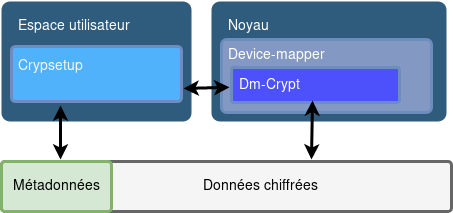
\includegraphics[width=.8\linewidth]{etat_art/organisation_linux.png}
\caption{\label{fig:OrgLinux}Organisation du code dans Linux}
\end{figure}

\paragraph{}
L'organisation reflétée par les programmes l'est également au niveau du code,
le module {\em dm-crypt} est agnostique de l'existance de métadonnées ainsi 
que de leur format. On a donc le module {\em device-mapper \em et \em dm-crypt}
qui font partie du code du noyau {\em Linux}, tandis que {\em Crypsetup} est un 
programme qui est usuellement fourni avec {\em Linux} en tant qu'utilitaire, 
qui est géré par une équipe indépendante de celle du noyau {\em Linux}. De plus 
{\em dm-crypt} est agnostique des algorithmes de chiffrement disponibles,
le module s'appuie sur l'API de cryptographie du noyau.

\paragraph{}
Dans le cas de {\em FreeBSD}, le module noyau qui est en charge des
transformations sur les disques est {\em GEOM}. Comme sous {\em Linux}, 
il existe des modules qui vont interagir avec GEOM pour fournir des fonction 
de RAID, de cache, et également de chiffrement. 
Ces modules sont appelés {\em Classes GEOM}, 
celle qui fournit le chiffrement est nommée {\em ELI}, le module noyau associé 
est ainsi appelé {\em GELI}. Le module contrairement à {\em dm-crypt}, 
comprend toute la logique des métadonnées, ainsi que des algorithmes de 
chiffrement disponibles. L'outil en espace utilisateur tire son code
directement du code du module {\em geli}. {\em GELI} profite de la 
connaissance du format des métadonnées pour directement détecter les 
partitions chiffrées, et donc proposer leur déchiffrement à l'utilisateur, 
là où {\em Linux} ne peut pas détecter de
partition ou disque chiffré, et c'est à l'utilisateur de préciser qu'il veut 
déchiffrer tel disque avec l'outil {\em crypsetup} qui va donc reconnaître le 
format. On a donc l'organisation suivante :


\paragraph{}
\begin{figure}[h]
\centering
\includegraphics[width=.8\linewidth]{etat_art/organisation_FreeBSD.png}
\caption{\label{fig:OrgFreeBSD}Organisation du code dans FreeBSD}
\end{figure}

\subsection{Format sur disque}
\paragraph{}
Le format sur disque désigne l'organisation des données et métadonnées sur le 
disque. L'idée générale étant de stocker sur une partie du disque les 
informations permettant de déchiffrer une autre partie du disque.
\paragraph{}
Comme le noyau {\em Linux} ne contient pas de format de métadonnées, 
c'est {\em Crypsetup} qui a choisi de créer un format appelé {\em Linux 
Unified Key Setup ({\em LUKS})}, comme format standard pour le chiffrement de 
disque sous {\em Linux}. En effet, {\em Crypsetup} implémente d'autres format 
de métadonnées comme {\em TrueCrypt} développé par la 
{\em TrueCrypt Fondation}. 
Le format {\em LUKS} consiste en des métadonnées au début de la partition, 
précédant les données chiffrées.

\paragraph{}
\begin{figure}[h]
\centering
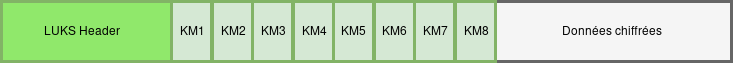
\includegraphics[width=.8\linewidth]{etat_art/format_disque_luks.png}
\caption{\label{fig:LUKSFormat}Format sur disque LUKS}
\end{figure}

\paragraph{}
Les métadonnées de {\em LUKS} contenant les algorithmes de chiffrement, 
d'authentification, la version de {\em LUKS}, sont suivis de huit emplacements 
permettant de stocker des clés chiffrées, qui permettent de déchiffrer le 
disque. Ainsi on peut stocker la même clé huit fois, protégées par des mots de 
passe différents, permettant ainsi à plusieurs utilisateurs de déchiffrer le 
même disque sans pour autant partager le même mot de passe.

\paragraph{}
Les métadonnées de {\em GELI} sont stockées contrairement à {\em LUKS}, 
à la fin du disque.
L'en-tête permet de stocker 2 clés, et s'étend sur un seul secteur.


\paragraph{}
\begin{figure}[h]
\centering
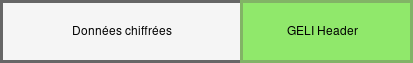
\includegraphics[width=.5\linewidth]{etat_art/format_disque_geli.png}
\caption{\label{fig:GELIFormat}Format sur disque GELI}
\end{figure}

\paragraph{}
Dans les deux en-têtes on retrouve des champs similaires, un {\em Magic} qui 
permet de connaître le type d'en-tête, la version, l'algorithme de chiffrement 
et d'authentification, etc. On peut noter tout de même que la taille de 
l'en-tête sous {\em GELI} fait 255 octets, contre 592 octets pour {\em LUKS}.



\subsection{Algorithmes}
\subsubsection{Algorithmes de chiffrement}
\paragraph{}
Les algorithmes de chiffrement disponibles pour {\em GELI} \cite{geli.h} sont :
\begin{itemize}
	\item Null
	\item Null-CBC
	\item AES-CBC
	\item AES-XTS
	\item Blowfish
	\item Blowfish-CBC
	\item Camellia
	\item Camellia-CBC
	\item 3DES
	\item 3DES-CBC
\end{itemize}

\paragraph{}
Dans le cas de {\em LUKS}, la spécification \cite{onDiskFormatLuks}
la liste des algorithmes disponibles, les noms des algorithmes ne sont pas 
interprétés par des opérations {\em LUKS}, mais pour des besoins de 
compatibilité avec d'autres implémentations, la liste des algorithmes 
disponibles est la suivante :
\begin{itemize}
	\item AES
	\item Twofish
	\item Serpent
	\item Cast5
	\item Cast6
\end{itemize}
Les algorithmes peuvent être associés aux modes suivants :
\begin{itemize}
	\item ECB
	\item CBC-plain
	\item CBC-essiv:hash
	\item XTS-plain64
\end{itemize}

\subsubsection{Utilisation de la clé primaire}
\paragraph{}
Dans le cas de {\em LUKS}, la spécification \cite{onDiskFormatLuks} précise 
que la clé stockée dans l'en-tête {\em LUKS} est utilisée directement comme 
clé de chiffrement. Dans le cas de {\em GELI}, la clé est dérivée selon un 
algorithme déterministe en des clés utilisées pour chiffrer les données, 
qui dépendent de la version de {\em GELI} et de l'utilisation 
d'authentification des données \cite{manGeli}. 
La version 5 de {\em GELI} utilisait une seule clé, qui était la clé
primaire fournie par les métadonnées, à partir de la version 6, la clé primaire
est dérivée en clés de chiffrement, qui diffèrent tout les 2\textasciicircum20 
secteurs, soit 1048576 secteurs du disques. Les tailles des secteurs des 
disques étant généralement de 512 octets ou 4096 octets, 
donc tout les 500Mo ou 4Go environ.
La taille du secteur correspond au champs taille du secteur des métadonnées
{\em GELI}.

\subsubsection{Algorithmes d'authentification (HMAC)}
\paragraph{}
Les algorithmes d'authentification disponibles sous {\em GELI} sont:
\begin{itemize}
	\item HMAC/MD5
	\item HMAC/SHA1
	\item HMAC/Ripemd160
	\item HMAC/SHA256
	\item HMAC/SHA384
	\item HMAC/SHA512
\end{itemize}

\paragraph{}
Dans le cas de {\em LUKS}, le chiffrement avec de l'authentification des 
données n'est pas supporté, cependant le service d'intégrité peut être rendu 
par le module {\em dm-verity} ou {\em dm-integrity}, le format des métadonnées 
est spécifié indépendamment de {\em LUKS}. Dans le cas où l'on souhaite faire 
du chiffrement et de l'authentification il est alors conseillé d'utiliser le 
module {\em dm-integrity}.

\subsubsection{Fonction pseudo aléatoire pour PBKDF2}
\paragraph{}
La spécification de PBKDF2 \cite{PKCS5v2} précise l'utilisation d'une fonction
pseudo aléatoire, dans le cas de {\em LUKS}, la spécification 
\cite{onDiskFormatLuks} liste les algorithmes autorisés
pour des raisons de compatibilité :
\begin{itemize}
	\item SHA1 (algorithme par défaut)
	\item SHA256
	\item SHA512
	\item Ripemd160
\end{itemize}
\paragraph{}
Dans le cas de {\em GELI}, c'est l'algorithme {\em SHA512} qui est utilisé
selon \cite{geliPkcs5v2.c}.
\subsection{Fonctionnalités}
\paragraph{}
Les deux systèmes de chiffrement : {\em dm-crypt \em et \em geli} profitent 
de l'accélération matérielle pour les opérations de chiffrement grâce au 
noyau (AES-NI notamment). {\em LUKS} supporte l'hibernation sur disque 
contrairement à {\em GELI}, qui ne le supporte pas car {\em FreeBSD} ne 
supporte pas l'hibernation sur disque. Les deux systèmes permettent le 
renforcement de phrases de passe, via la fonction {\em PBKDF2} décrite 
par le standard {\em PKCS\#5v2}. Les deux formats de métadonnées 
permettent l'utilisation de plusieurs clés.

\subsubsection{Intégration avec la séquence de démarrage}
\paragraph{}
L'intégration avec le démarrage permet notamment d'avoir la racine du système 
de fichier sur une partition chiffrée, et même éventuellement le {\em /boot}
dans lequel sont usuellement stockés les fichiers permettant de démarrer le 
système d'exploitation.

\paragraph{}
Dans le cas de {\em Linux}, le format {\em LUKS} a été intégré dans
l'initramfs via un hook qui charge le module {\em dm-crypt} puis utilise 
le binaire {\em cryptsetup} pour déchiffrer le disque. 
Le format {\em LUKS} a également été intégré à {\em GRUB} sous la 
forme du module {\em luks.mod}. Il permet au premier stage de {\em GRUB} de 
déchiffrer la partition sur laquelle se trouve la configuration de {\em GRUB}.
Ainsi sous {\em Linux}, il est possible de chiffrer toute la racine de son 
système, {\em /boot} compris. Il est ensuite question de pouvoir taper une 
seule fois la phrase de passe, 
pouvoir faire de l'authentification unique (SSO), cela est 
également possible, il suffit de mettre un fichier contenant la clé de 
chiffrement en clair dans l'initramfs. Ainsi {\em GRUB} déchiffre le disque, 
puis charge l'initramfs qui peut déchiffrer la partition sans avoir besoin 
de demander une phrase de passe.

\paragraph{}
Dans le cas de {\em GELI}, il est également possible de chiffrer la racine du 
système, le bootloader de {\em FreeBSD} étant capable de lire les métadonnées 
{\em GELI}, ainsi que de déchiffrer des données. 
Il est également possible de chiffrer le 
{\em /boot} car le 2ème stage du bootloader ({\em boot2}) contient le code 
nécessaire pour déchiffrer un disque au format {\em GELI}, à condition que 
la table de partition soit au format GPT. La phrase de passe est passée via 
une zone mémoire au dernier stage qui pourra l'utiliser pour démarrer.



% Chapitre 2: Description du projet et des choix de développement
\chapter{Choix de développement}

\section{Les métadonnées}
\subsection{Utilisation des métadonnées stockées sur le disque dans le code
source de GELI}
\label{ssec:md_usage}
L'analyse de \textit{LUKS} et \textit{GELI} nous a montré les similitudes et
différences que présentent ces deux systèmes.
\paragraph{}
\begin{figure}[h]
\centering
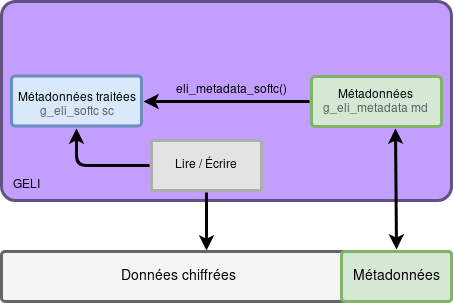
\includegraphics[width=.6\linewidth]{choix_developpement/utilisation_metadonnee.png}
\caption{\label{fig:softc_eli}Métadonnées en mémoire}
\end{figure}

\paragraph{}
Pour n'importe-quel module noyau utilisant la classe \textit{GEOM} de
\textit{FreeBSD}, les métadonnées sont toujours placées à la fin des données du
disque, contrairement à \textit{LUKS}. Il faut donc créer les fonctions
utilisant celles fournies par \textit{GEOM} afin de réaliser cette opération.
\paragraph{}
Dans le cas d'un fichier (utile pour sauvegarder l'en-tête contenant les 
métadonnées), il suffit d'utiliser les fonctions standards de
\verb|C| et de lire le début du fichier. Dans le cas d'un disque en revanche, il
faut créer une fonction lisant les premiers secteurs. On peut ensuite les
stocker dans une structure afin de connaître les propriétés de chiffrement
utilisées.

\paragraph{}
Les informations présentes dans les métadonnées \textit{LUKS} sont assez proches
de celles de \textit{GELI}:
\begin{itemize}
\item le \textit{MAGIC}
\item la version utilisée
\item l'algorithme de chiffrement
\item l'algorithme de hashage
\item le sel
\item le nombre d'itérations PKCS
\item la \textit{masterkey} chiffrée
\end{itemize}

\paragraph{}
Les métadonnées sont donc stockées sur le disque et sont mappées en mémoire via
la structure {\em md} de type {\em g\_eli\_metadata}. Mais des métadonnées 
"indirectes" sont aussi présentes en mémoire à travers la structure {\em softc} 
de type {\em g\_eli\_softc}. Comme illustré par le schéma \ref{fig:softc_eli} 
cette structure diffère des 
métadonnées à proprement parler. En effet les métadonnées évoquées jusqu'ici sont
celles qui sont stockées telles quelles sur le disque à l'encodage près. Les 
données privées de l'instance GEOM sont stockées dans une structure présente 
uniquement en mémoire et dont les champs sont remplis par les métadonnées du 
disque, mais aussi par des informations sur le disque comme sa taille ou encore 
la taille des secteurs. Enfin les clés de chiffrement qui sont dérivées à partir
de la clé maître y sont également stockées sous la forme d'un arbre et d'une 
queue.

\subsection{Transformer les métadonnées de LUKS en métadonnées GELI}
\subsubsection{Principe général}
\paragraph{}
Écrire un module noyau de toute pièce capable d'utiliser un disque chiffré avec
\textit{LUKS} serait une tâche très longue. Sachant que de nombreuses fonctions
s'inspireraient du module \textit{GELI}, il est préférable de reprendre le code
(sous license \underline{BSD-2-Clause-FreeBSD}) et de l'adapter à la lecture et
l'écriture de données sur un disque chiffré \textit{LUKS}. Cependant, les
fonctions étant extrêmement dépendantes de la structure des métadonnées, dont
l'usage globale est visible sur la \textit{Figure \ref{fig:fonctions_md}};
19.35\% des fonctions dépendent de cette structure. Cette utilisation se fait
également à travers la structure \texttt{softc}, utilisée par 44.09\% des
fonctions (\textit{Figure \ref{fig:fonctions_sc}}), qui désigne les données
privées de l'instance GEOM. Leur modification équivaudrait à une refonte assez
importante du code.
\paragraph{}
\begin{figure}[h]
\centering
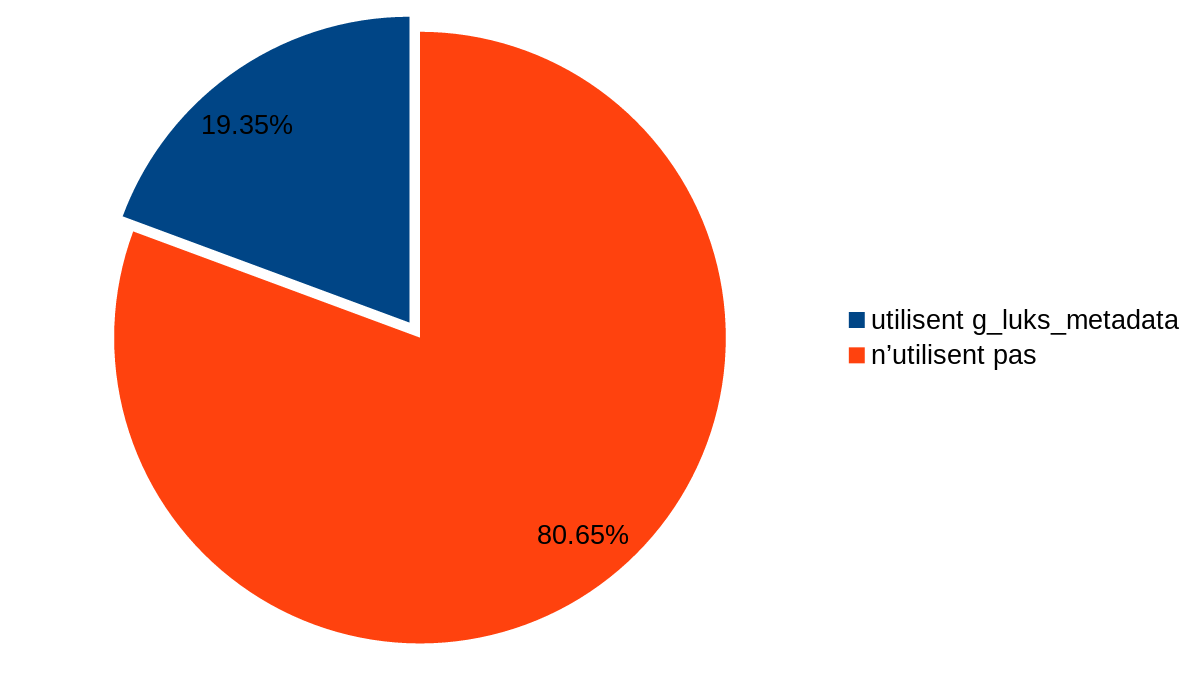
\includegraphics[width=.9\linewidth]{choix_developpement/fonctions_g_luks_metadata.png}
\caption{\label{fig:fonctions_md}Fonctions utilisant les métadonnées}
\end{figure}
\paragraph{}
\begin{figure}[h]
\centering
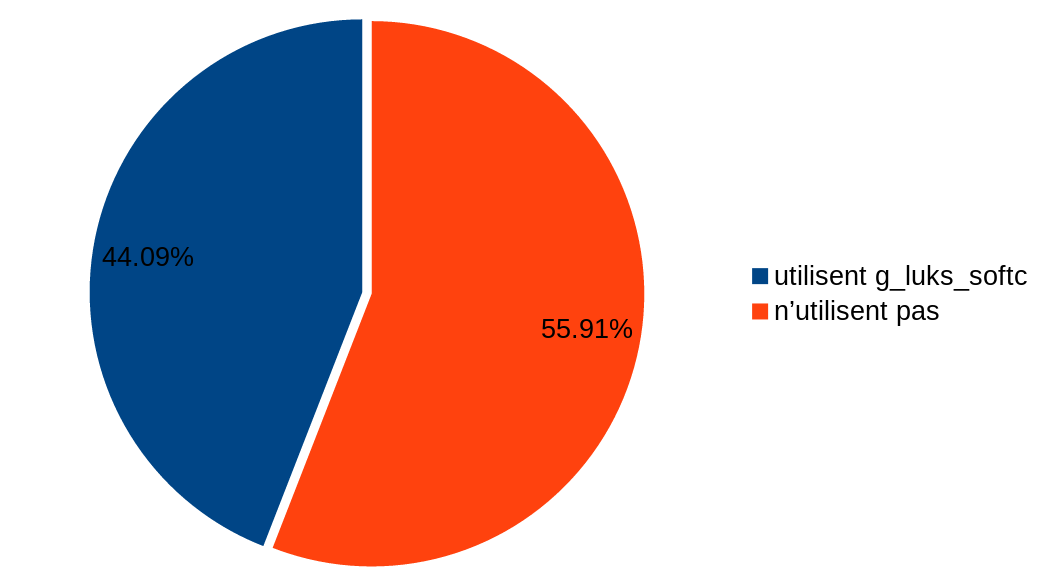
\includegraphics[width=.9\linewidth]{choix_developpement/fonctions_g_luks_softc.png}
\caption{\label{fig:fonctions_sc}Fonctions utilisant la structure \texttt{softc}}
\end{figure}
\paragraph{}
C'est pourquoi, la solution la plus intéressante serait de garder la structure
de \textit{GELI} et d'y mettre les informations de chiffrement. Cela permettra 
notamment d'écrire et/ou de modifier moins de code et donc de limiter les erreurs
et de faciliter la maintenabilité. De plus en choisissant de procéder ainsi, on
peut modifier le code facilement par itérations en le gardant compilable et 
exécutable. On choisit donc de conserver le code de 
GELI le plus possible et de transformer les métadonnées de LUKS en métadonnées 
GELI.

\paragraph{}
En effet bien que les métadonnées stockées sur le disque soient différentes 
entre GELI et LUKS, le chiffrement du disque reste essentiellement identique :
on utilise une clé maître et un algorithme de chiffrement de blocs. Cependant 
comme décrit auparavant, la clé maître dans GELI est dérivée en clés de 
chiffrement. Toutefois, GELI laisse la possibilité à travers des {\em Flags} 
d'utiliser la clé maître comme unique clé de chiffrement.

\paragraph{}
Comme décrit en \ref{ssec:md_usage}, les métadonnées utilisées par l'instance
GEOM sont celles qui sont stockées dans la stucture {\em softc}, à l'exception
de la lecture sur disque des métadonnées et de leur vérification ainsi que le 
changement des métadonnées sur le disque (changement de la phrase de passe et
donc de la clé chiffrée sur le disque).

\paragraph{}
\begin{figure}[h]
\centering
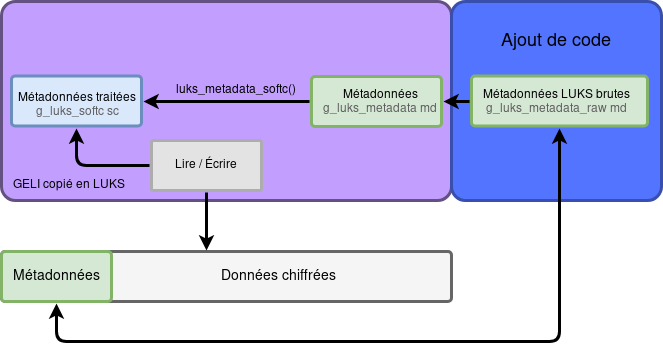
\includegraphics[width=.9\linewidth]{choix_developpement/utilisation_metadonnee_luks.png}
\caption{\label{fig:transformation_md}Transformation des métadonnées}
\end{figure}

\paragraph{}
La transformation des métadonnées LUKS en métadonnées GELI consiste donc à 
remplacer la lecture des métadonnées du disque par GELI par celles de LUKS 
comme illustré par le schéma \ref{fig:transformation_md}. On change donc la 
fonction {\em luks\_metadata\_softc} pour qu'elle utilise les données extraites
de l'en tête LUKS du disque au lieu de celles extraites de l'en tête GELI, donc
respectivement du premier secteur et de quelques secteurs suivant au lieu du 
dernier secteur. On devra également changer la gestion du déchiffrement de la 
clé du disque.


\subsubsection{Déchiffrement de la clé de chiffrement dans le cas de GELI}
Dans le cas de GELI, le code prévoit le déchiffrement de la clé de chiffrement 
dans le noyau, de façon à pouvoir déchiffrer le disque au démarrage (pour 
pouvoir avec un volume racine chiffré). Plus précisément l'utilitaire en espace
utilisateur envoie au noyau via l'API de GEOM, la phrase de passe dérivée via
l'algorithme PKCS5v2 en prenant SHA512 comme fonction pseudo aléatoire.


\subsubsection{Déchiffrement de la clé de chiffrement dans le cas de LUKS}
\paragraph{}
On a donc besoin de déchiffrer la clé de chiffrement stockée dans l'en-tête LUKS.
Pour cela il faut tout d'abord bien comprendre comment est stockée la clé de 
chiffrement sur le disque.

\paragraph{}
La clé de chiffrement est hashée selon l'algorithme spécifiée par le champ
{\em hash-spec}, et stockée dans le champ {\em mkdigest} (Master Key Digest).

L'en-tête LUKS permet de stocker la même clé chiffrée avec huits phrases de passe
différentes, dans les huits {\em KeySlot} définis par le standard.
\\
Pour un keyslot, la phrase de passe est dérivée selon l'aglorithme {\em PKCS5v2}
avec comme fonction pseudo aléatoire l'algorithme de hashage spécifié par 
{\em hash-spec}. La clé est ensuite fragmentée via l'algorithme 
{\em anti-forensic splitter} spécifié dans \cite{AFsplitting} qui a pour but de
lutter contre la persistance des informations stockées sur des disques dur
(disques qui utilisent le magnétisme pour stocker les données)
\\
Enfin le résultat de la fragmentation est chiffré selon l'algorithme utilisé 
pour les données du disque (donc précisé par les champs {\em cipher-name} et 
{\em cipher-mode}) avec comme clé le résultat de la dérivation de la phrase de
passe.

\paragraph{}
Une différence avec {\em GELI} est que le nombre d'itérations utilisée pour 
{\em PKCS5v2} est différent pour chaque keyslot alors que pour {\em GELI} c'est
le même pour toutes les phrases de passe.
Dans {\em GELI} la phrase de passe est dérivée en espace utilisateur avant 
d'être envoyée en espace noyau, qui déchiffrera ensuite la clé de chiffrement.
Or si l'on applique le même procédé pour {\em LUKS}, il faut alors dans le cas
où les 8 keyslot sont actifs, envoyer 8 phrases de passe dérivées au noyau.
Il est donc plus simple d'envoyer la phrase de passe directement au noyau, qui
effectuera donc tout les calculs.

\subsubsection{Sélection des algorithmes utilisés}
\paragraph{}
Deux données importantes sont nécessaires pour le chiffrement et déchiffrement
de disque: l'algorithme de chiffrement utilisé ainsi que la méthode de
génération du vecteur d'initialisation \textbf{IV}. Dans notre cas, l'algorithme
de chiffrement peut être \textbf{aes-xts}, \textbf{aes-cbc} ou
\textbf{cast5-cbc}. Chacun de ces algorithmes n'accepte pas les même méthodes de
génération de l'\textbf{IV}, qui peut être de type \textit{plain} (32 ou 64) ou
\textit{essiv:sha256}. Le vecteur d'unitialisation est unique à chaque secteur
du volume chiffré. Le premier type prend numéro du secteur concerné codé sur 32
ou 64 bits comme vecteur d'initialisation, tandis que \textit{essiv:sha256}
(pour \textbf{e}ncrypted \textbf{s}ector-\textbf{s}alt \textbf{i}nitialization
\textbf{v}ector) calcule l'IV à partir d'une combinaison du numéro de secteur
avec le hachage de la clé de chiffrement.
\paragraph{}
\begin{figure}[h]
\centering
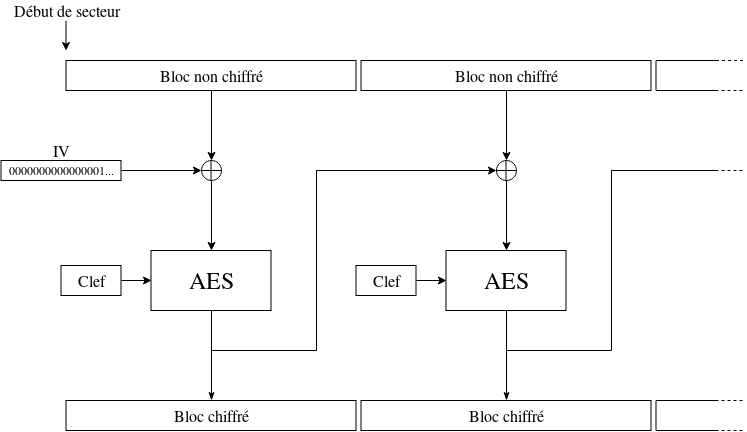
\includegraphics[width=.9\linewidth]{choix_developpement/aes_cbc.png}
\caption{\label{fig:aes_cbc}Chiffrement en AES-CBC}
\end{figure}
\paragraph{}
Dans les métadonnées \textit{LUKS}, deux champs distincts permettent à
\textit{dm-crypt} de connaitre l'algorithme de chiffrement utilisé ainsi que la
manière dont le vecteur d'initialisation \texttt{IV} est calculé:
\begin{itemize}
\item \textbf{Cipher name}: nom de l'algorithme de chiffrement utilisé
\item \textbf{Cipher mode}: manière dont le vecteur d'initialisation est généré
\end{itemize}
\paragraph{}
Dans les métadonnées \textit{GELI}, ces deux informations sont confondues dans
le champs \textbf{ealgo} (\textit{encryption algorithm}). La variable est
ensuite enregistrée et utilisée dans la structure \texttt{softc}. Le calcul de
\textbf{IV} quant à lui est géré par la fonction \texttt{g\_eli\_crypto\_ivgen},
qui est soit en mode \textit{plain64} lorsque l'algorithme \textbf{aes-xts} est
utilisé, et \textit{essiv:sha256} autrement.
\paragraph{}
Par défaut, le type d'\textbf{IV} (le \texttt{cipher mode} dans \textit{LUKS})
calculé par la fonction de \textit{GELI} dépend de l'algorithme de chiffrement
(le \textit{cipher name} dans \textit{LUKS}). Cette y association est codée en
dur:
\begin{itemize}
\item le calcul de l'\textbf{IV} est équivalent au mode \texttt{plain64} de
  \textit{LUKS} lorsque l'algorithme \textbf{AES-XTS} est indiqué
\item le calcul correspond au mode \texttt{essiv:sha256} de \textit{LUKS}
  autrement
\end{itemize}
\paragraph{}
Il est donc nécessaire d'adapter la fonction afin qu'elle prenne en compte les
propriétés indiquées dans les métadonnées \textit{LUKS} lorsqu'elles sont mises
au format \textit{GEOM ELI}. Il n'est cependant pas possible d'utiliser
directement tous les algorithmes et modes possibles avec \textit{LUKS} sans
modifier les structures \texttt{metadata} et \texttt{softc} hériftées de
\textit{GELI}. Ces structures étant utilisées par de nombreuses fonctions, leur
modification nécessiterait celle d'une très grande partie du code. Le nombre de
choix possibles est donc limité aux associations suivantes:
\begin{center}
  \begin{tabular}{ | l | l | }
    \hline
    \textbf{Cipher name} & \textbf{Cipher mode}  \\
    \hline
    AES-XTS              & \texttt{plain64}      \\
    AES-CBC              & \texttt{essiv:sha256} \\
    CAST5-CBC            & \texttt{plain}        \\
    \hline
  \end{tabular}
\end{center}


% Chapitre 3: Difficultés rencontrées
\chapter{Difficultés rencontrées}

\section{Développement noyau et débogage}

\subsection{Développement noyau}

\paragraph{}Nous avons du implémenter la majorité des fonctions dans le code du
module noyau que nous avons créé à partir de {\em GELI}. Il a donc fallu se
familiariser avec les différences entre noyau et espace utilisateur, on peut
par exemple citer l'allocation dynamique ou encore les fonctions de chiffrement
et de déchiffrement qui diffèrent.

\paragraph{}
Dans l'espace utilisateur la bibliothèque {\em Openssl} fournit la plupart des
fonctions de chiffrement et de hashage, tandis que dans le noyau nous avons du
utiliser l'API {\em Opencrypto}. De même, nous avons du nous familiariser avec
l'API que propose {\em GEOM} pour comprendre les différents champs des
structures et fonctions utilisées.

\subsection{Débogage}
\paragraph{}
L'une des plus grosse difficultés provenait du fait, qu'en mode noyau,
peu d'erreurs sont permises. Par exemple nous avons souvent du faire face à
des erreurs de page ou des débordements mémoire qui ne sont alors pas
rattrapables par le noyau, qui causait alors un plantage du noyau. Nous avons
tout de même pris soin d'activer le débogage noyau dans FreeBSD, ce qui nous
permettaient de récupérer une image mémoire du noyau que l'on pouvait exploiter
ultérieurement avec un débogueur noyau.

\paragraph{}Dans les cas où il n'y avait pas de plantage, l'utilisation de
{\em printf} nous permettait de déboguer le programme en affichant la valeur
de certaines variables, qui apparaissaient alors dans les messages envoyées par
le noyau, que l'on peut consulter avec la commande {\em dmesg} sous la majorité
des systèmes UNIX dont FreeBSD.






% Chapitre 4: Utilisation
\chapter{Utilisation de GEOM\_LUKS}

\section{Compatibilité entre Linux et FreeBSD}

\subsection{Le système de fichiers}
Nous avons donc implémenté une première version d'un module noyau et de son
utilitaire pour FreeBSD qui permet la lecture et l'écriture sur un volume chiffré
avec le format LUKS1.0. La version 2.0 de LUKS est encore en développement,
pour arriver à sa version finale, bien que déjà disponible sous Linux. Pour
pouvoir utiliser la partition au format LUKS sous FreeBSD il faut un système de
fichiers qui soit supporté par les deux systèmes d'exploitation. En listant
les systèmes de fichiers disponibles, on peut noter que {\em EXT2, EXT3, openZFS,
FAT, FAT32, et NTFS} sont disponibles sous Linux et FreeBSD. Le support de {\em
XFS} a été retiré avec FreeBSD 10 et celui de {\em EXT4} n'existe actuellement
qu'en lecture seule.

\subsection{Le démarrage}
Nous n'avons pas implémenté la partie s'occupant du démarrage sur une partition
chiffrée avec {\em LUKS}. Cependant pour démarrer sur un système dans lequel le
{\em /boot} est séparé, il suffirait de peu de modifications du code actuel pour
permettre au noyau, lors de son chargement, d'ouvrir le \texttt{/} chiffré avec
{\em LUKS}. Le fonctionnement du point de vue de l'utilisateur serait ainsi
semblable à un système chiffré avec {\em GELI}.

\subsection{Partage de fichiers et haute disponibilité}
\paragraph{}
On peut donc imaginer des cas d'utilisation de {\em LUKS} sous FreeBSD
permettant par exemple de partager des fichiers entre Linux et FreeBSD, et donc
de faciliter l'installation de {\em dual-boot} Linux-FreeBSD. On peut également
imaginer disposer de systèmes Linux et FreeBSD pour réaliser la même opération
sur un stockage réseau qui serait chiffré avec {\em LUKS}, permettant
d'accroître la disponiblité du système en utilisant deux systèmes d'exploitation
différents tout en conservant la propriété de confidentialité, en permettant
uniquement à la machine qui utilise le disque de pouvoir le lire (et donc
interdisant la machine hébergeant le disque de pouvoir lire son contenu).
\paragraph{}
Le partage de médias amovibles chiffrés avec \textit{LUKS} est également rendu
possible entre les deux systèmes. Une simple clé USB ou un disque dur externe
pourraient alors être chiffrés, en gardant la capacité d'être lus et écrits par
les deux systèmes, sans modification particulière faite au préalable.


% Chapitre 5: Tests
\chapter{Tests}

\paragraph{}
L'ensemble des tests ont été réalisés via l'utilisation de machines virtuelles,
mais ils auraient pu être reproduits sur de vraies machines.

\section{Mise en place}

\paragraph{}
Dans le but de correctement tester la compatibilité entre les deux systèmes, il
est nécessaire d'installer chacun d'eux, de telle sorte qu'ils aient un disque
en commun.

\subsection{Installation des systèmes}
\subsubsection{Linux}
Le système Linux utilisé peut être n'importe-quelle distribution, tant qu'il est
possible d'y gérer des disques chiffrés avec le standard \textit{LUKS 1}. Pour
cela, il est nécessaire que \texttt{cryptsetup} soit installé. La machine ne
servira ensuite plus qu'à créer les volumes chiffrés avec différents algorithmes
afin de tester leur déchiffrement depuis FreeBSD.
\subsubsection{FreeBSD}
Nous nous sommes basé sur la dernière version stable de FreeBSD à ce jour, à
savoir la version \textit{11.2-RELEASE}. Il est directement possible d'y
compiler un nouveau noyau ainsi que ses utilitaires à partir du code source.

\subsection{Création des partions chiffrées}
\paragraph{}
Les partitions chiffrées sont créées depuis le système Linux sur un disque
séparé et enregistré en tant qu'image disque virtuelle. Les partitions créées
sont:
\begin{itemize}
\item une partition chiffrée \texttt{aes-xts-plain64}
\item une partition chiffrée \texttt{aes-cbc-plain}
\item une partition chiffrée \texttt{aes-cbc-essiv:sha256}
\item une partition chiffrée \texttt{cast5-cbc-plain}
\item une partition en clair
\end{itemize}
\paragraph{}
Après avoir créé différentes partitions à l'aide d'un outils comme
\texttt{cfdisk}, il est possible d'y créer un système chiffré LUKS. Les
commandes utilisées afin de créer les différentes partitions chiffrées sous
Linux sont:
\\
\begin{lstlisting}[language=bash]
  # Linux
  
  cryptsetup luksFormat -c aes-xts-plain64 /dev/sdb1
  cryptsetup luksFormat -c aes-cbc-plain /dev/sdb2
  cryptsetup luksFormat -c aes-cbc-essiv:sha256 /dev/sdb3
  cryptsetup luksFormat -c cast5-cbc-plain /dev/sdb4
\end{lstlisting}
\paragraph{}
Il est ensuite possible de déchiffrer les partitions pour les formater et y
écrire des données. Cela permettra de vérifier par la suite que notre
implémentation de \textit{LUKS} sur FreeBSD est bien capable de le lire.
\\
\begin{lstlisting}[language=bash]
  # Linux
  
  cryptsetup luksOpen /dev/sdb1 luks_device
  mkfs.ext2 /dev/sdb1 # necessaire qu'au moment de la creation du volume
  mount /dev/mapper/luks_device /mnt
  echo "geom_luks: aes-xts-plain64 OK" > /mnt/file.txt
  umount /mnt
  cryptsetup luksClose luks_device
\end{lstlisting}
\paragraph{}
Une fois les partitions chiffrées créées sur un disque, on peut l'ajouter à la
machine fonctionnant sous FreeBSD, qui pourra ainsi directement interagir
directement avec lui.
\paragraph{}
Pour plus de simplicité mais des tests équivalents, il est également possible
d'utiliser des fichiers et d'y héberger les systèmes chiffrés. Cette opération
est réalisable sous Linux cette manière:
\\
\begin{lstlisting}[language=bash]
  # Linux
  
  # creation du fichier
  dd if=/dev/zero of=file bs=1M count=10
  losetup -a /dev/loop0 file
  cryptsetup luksFormat -c aes-xts-plain64 /dev/loop0
  cryptsetup luksOpen /dev/loop0 luks_device
  mkfs.ext2 /dev/mapper/luks_device

  # effectuer les actions voulues sur /dev/loop0
  # (dechiffrement, montage, lecture, ecriture, ...)

  cryptsetup luksClose luks_device
  losetup -d /dev/loop0
\end{lstlisting}
\paragraph{}
Une fois les partitions créées et formatées, seule la commande
\texttt{cryptsetup luksOpen} est nécessaire avant de monter le volume. Chacune
de ces partitions contient un système de fichiers \texttt{ext2}, lisible
directement sur FreeBSD grâce au module noyau \textit{Ext2fs} via la commande
\texttt{mount -t ext2fs /dev/ada1p1 /mnt} (\texttt{/dev/ada1p1} étant
l'emplacement du volume à monter dans \texttt{/mnt/}; figure
\ref{fig:linux_partitions}).
\begin{figure}[H]
  \centering
  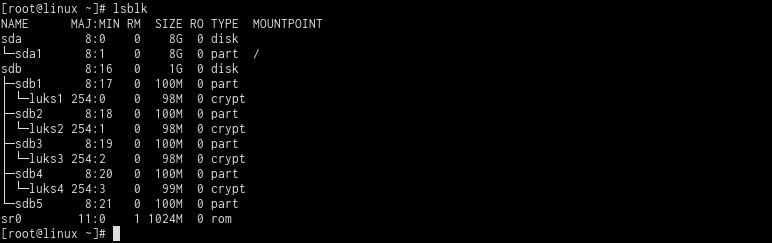
\includegraphics[width=\linewidth]{tests/linux_partitions.png}
  \caption{\label{fig:linux_partitions}Création des partitions}
\end{figure}
Dans le cas où on utilise d'un fichier qu'on aurait copié dans le répertoire
courant, il faut d'abord l'attacher en tant que disque avec l'outil
\texttt{mdconfig}.
\\
\begin{lstlisting}[language=bash]
  # FreeBSD
  
  # attacher le fichier
  mdconfig -a file -u 0

  # detacher le fichier
  mdconfig -d -u 0
\end{lstlisting}
\paragraph{}
\texttt{-u 0} permet d'indiquer que l'emplacement \texttt{/dev/md0} sera
utilisé.

\section{Tests des différentes fonctionnalités}

\subsection{Lecture des métadonnées}
\paragraph{}
Dans un premier temps, afin de tester la lecture de métadonnées sans devoir se
préocuper des difficultés posées par la lecture de disque (notamment dues à
l'emplacement des métadonnées qui diffère entre \textit{LUKS} et \textit{GELI}),
nous avons créé des fichiers contenant un volume chiffré. Pour ce faire, on
copie dans un fichier les données d'une des partitions chiffrées \textit{LUKS}
créées précédemment. Cette opération est directement réalisée sur FreeBSD. On
tente ensuite d'afficher les métadonnées présentes sur ce fichier.
\\
\begin{lstlisting}[language=bash]
  # Linux

  cryptsetup luksDump /dev/sdb1
\end{lstlisting}
\begin{lstlisting}[language=bash]
  # FreeBSD
  
  dd if=/dev/ada1p1 of=file bs=1M
  gluks dump_raw file
\end{lstlisting}
\paragraph{}
Cela permet de vérifier que la structure utilisée est cohérente et que les types
de ses variables sont corrects. Pour cela, on utilise les commandes réalisant
cette opérations et on compare leur sortie sur les deux systèmes (figures
\ref{fig:linux_dump_file} et \ref{fig:freebsd_dump_file}).
\begin{figure}[H]
  \centering
  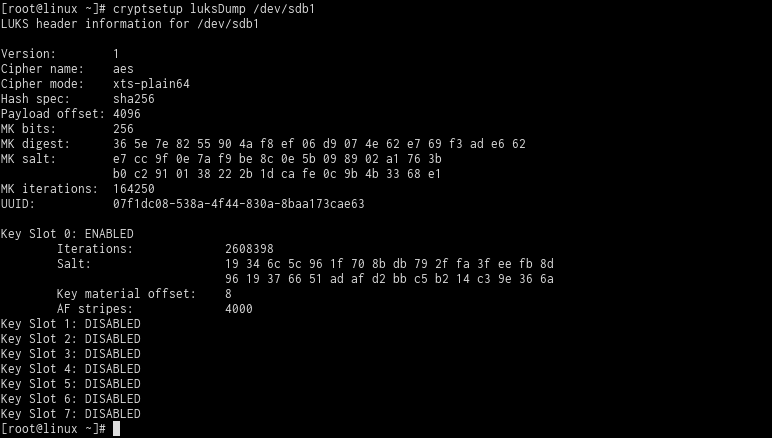
\includegraphics[width=\linewidth]{tests/linux_dump_disk.png}
  \caption{\label{fig:linux_dump_file}Affichage des métadonnées sur Linux}
\end{figure}
\begin{figure}[H]
  \centering
  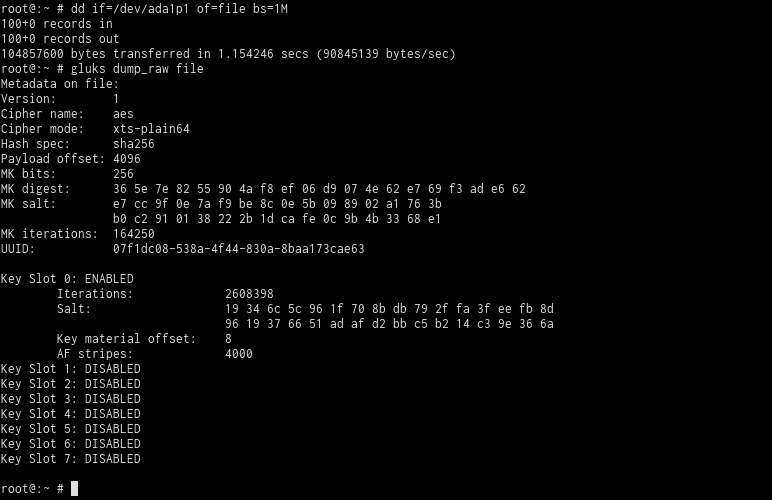
\includegraphics[width=\linewidth]{tests/freebsd_dump_file.png}
  \caption{\label{fig:freebsd_dump_file}Affichage des métadonnées sur FreeBSD
    depuis un fichier}
\end{figure}

\paragraph{}
Une fois que la structure des métadonnées utilisée a été vérifiée et validée, on
peut poursuivre les tests sur une \textit{vraie} partition chiffrée. Pour ce
faire, on peut utiliser les partitions chiffrées \textit{LUKS} qui sont
accessibles depuis notre système FreeBSD (figure \ref{fig:freebsd_dump_disk}).
\\
\begin{lstlisting}[language=bash]
  # FreeBSD

  gluks dump_raw /dev/ada1p1
\end{lstlisting}
\begin{figure}[H]
  \centering
  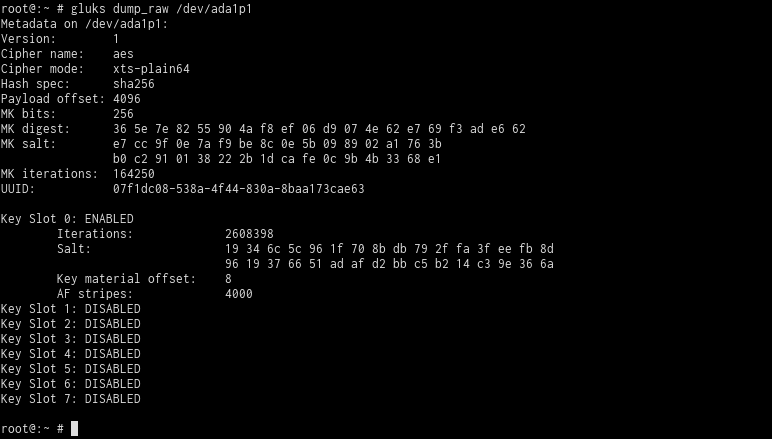
\includegraphics[width=\linewidth]{tests/freebsd_dump_disk.png}
  \caption{\label{fig:freebsd_dump_disk}Affichage des métadonnées sur FreeBSD
    depuis un disque}
\end{figure}

\subsection{Déchiffrement de la clé maître}
\paragraph{}
Pour tester le déchiffrement de la clé maître (ou \textit{masterkey}), on part
de la fonction \texttt{geli attach}, responsable du déchiffrement et de
l'attachement d'un volume chiffré, en enlevant dans un premier temps la partie
de la fonction s'occupant de l'attachement.
\paragraph{}
Sous FreeBSD, l'attachement de volume avec \textit{GELI} consiste en son
déchiffrement et le fait de le rendre disponible au montage. Une fois déchiffré,
un fichier ayant pour extension \texttt{.eli} (ou \texttt{.luks} dans notre
outil) est créé: c'est lui qui pourra ensuite être monté comme n'importe-quel
autre volume non chiffré. Sur un système Linux, ce fichier correspond à celui
créé dans \texttt{/dev/mapper/} grâce à \texttt{cryptsetup luksOpen}. Cette
opération est donc ignorée pour l'instant.
\paragraph{}
Les fonctions réalisant le déchiffrement de la clé maître à partir d'une phrase
secrète permettent de savoir si celle-ci est correcte où non. Il est donc
possible de savoir si le déchiffrement se fait correctement, sans même avoir
besoin de monter le disque pour vérifier son contenu (figure
\ref{fig:freebsd_test_passphrase}).
\\
\begin{lstlisting}[language=bash]
  # FreeBSD

  gluks test_passphrase /dev/ada1p1
\end{lstlisting}
\begin{figure}[H]
  \centering
  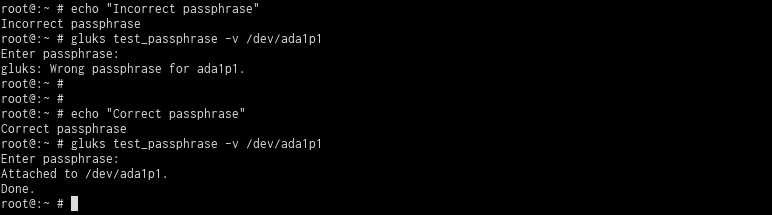
\includegraphics[width=\linewidth]{tests/freebsd_test_passphrase.png}
  \caption{\label{fig:freebsd_test_passphrase}Test de déchiffrement de la clé maître}
\end{figure}
\paragraph{}
Dans le premier cas, une phrase secrète incorrecte a été entrée. Le système
n'arrivant pas à déchiffrer la clé maître à partir de cette phrase, il a donc
pas attaché le volume.
\paragraph{}
Dans le second cas, la phrase entrée était correcte. Le système a donc pu
déchiffrer la clé maître et a attaché le volume, en créant un fichier
d'extension \texttt{.luks}.

\subsection{Montage et lecture de données}
\paragraph{}
Maintenant qu'il est possible de déchiffrer la clé maître, responsable du
chiffrement du disque, à partir d'une des phrases secrètes, il faut s'assurer du
bon déchiffrement du disque en tant que tel.
\paragraph{}
On reprend la fonction précédente pour y ajouter cette fois-ci la partie
responsable de l'attachement du volume chiffré. Après s'être assuré qu'un
fichier en \texttt{.luks} est bien créé dans \texttt{/dev/}, son montage dans
l'arborescence peut se faire. On peut ensuite s'assurer de son contenu, en
vérifiant par exemple celui d'un fichier texte qui a été créé sous Linux.
\\
\begin{lstlisting}[language=bash]
  # FreeBSD

  gluks test_passphrase /dev/ada1p1
  mount -t ext2fs /dev/ada1p1.luks /mnt
  
  cat /mnt/file.txt # ecrit "geom_luks: aes-xts-plain64" sur la sortie standard

  unmount /mnt
  gluks detach /dev/ada1p1
\end{lstlisting}
% TODO: figure cat

\subsection{Montage et écriture de données}
\paragraph{}
De même, une fois le volume déchiffré monté, il doit être possible d'y écrire
des données. On peut par exemple y placer un fichier contenant du texte.
\paragraph{}
Il est ensuite possible de vérifier son contenu depuis notre machine Linux, en
ouvrant le disque avec \texttt{cryptsetup} puis en le montant.
\\
\begin{lstlisting}[language=bash]
  # FreeBSD

  gluks test_passphrase /dev/ada1p1
  mount -t ext2fs /dev/ada1p1.luks /mnt
  
  cat /mnt/file.txt # ecrit "geom_luks: aes-xts-plain64" sur la sortie standard

  unmount /mnt
  gluks detach /dev/ada1p1
\end{lstlisting}
% TODO: figure echo in FreeBSD, cat in Linux

\subsection{Déchiffrement de disque avec différentes phrases secrètes}
\paragraph{}
Dans le stardard \textit{LUKS} comme dans \textit{GELI}, il est possible de
déchiffré une partition avec différentes phrases secrètes. Cela est réalisé dans
\textit{LUKS} en utilisant 8 \texttt{slots} prévus à cet effet, chacun
correspondant à une phrase.
Pour ajouter et enlever une phrase de déchiffrement à un disque, on utilise les
commandes suivantes:
\\
\begin{lstlisting}[language=bash]
  # Linux

  cryptsetup luksAddKey /dev/sdb1
  cryptsetup luksRemoveKey /dev/sdb1
\end{lstlisting}
Il est ainsi possible de retrouver dans des cas où les \texttt{slots} actifs ne
sont pas consécutifs.
% TODO: figure medatata 2 passphrases
\paragraph{}
Afin de tester que le déchiffrement se fait correctement pour chaque phrase
secrète, on reproduit les tests précédents pour chacune d'entre-elles.

% Chapitre 5: Tests
\chapter{Conclusion}
\section{Module noyau et utilitaire GEOM\_LUKS}

\paragraph{}
Pour l'instant le module noyau et l'utilitaire développés supportent l'ouverture
d'un disque chiffré avec {\em LUKS}, et donc l'écriture et la lecture d'un
volume qui est chiffré avec le standard. Cependant le module ne supporte
actuellement pas le standard dans son intégralité.

%TODO: Ecrire un paragraphe ou tableau ou liste de ce qu'il manque ou ce qu'on a en fonction de ce qui est le plus court

\section{Suite du projet}
\paragraph{}
Pour arriver à pouvoir intégrer le module noyau et l'utilitaire dans la branche
principale de FreeBSD, il reste cependant quelques étapes essentielles. Il
faudrait probablement dans un premier temps factoriser le code, enlever les
fonctions de {\em GELI} qui ne sont plus utiles, simplifier les fonctions en
enlevant le code qui était utile sous {\em GELI} mais ne l'est plus sous
{\em GLUKS}, on peut citer notamment tout ce qui est en rapport avec
l'authentification des données sur le disque, ou encore les fonctions s'occupant
de la dérivation de la clé de chiffrement. Par la suite, on pourrait modifier,
voire se passer des structures \texttt{g\_luks\_metadata} et
\texttt{g\_luks\_softc} héritées de {\em GELI} pour n'utiliser que celles de
{\em GLUKS}. Il faudrait également développer les scripts de tests, probablement
en adaptant ceux de {\em   GELI}, car l'utilitaire {\em geom\_luks} est très
proche de {\em geom\_eli}. Enfin il faudrait s'assurer du respect des
conventions de style de FreeBSD pour le noyau, et faire réaliser une revue de
code par les développeurs de FreeBSD.

\paragraph{}
Concernant l'utilitaire, il permet actuellement d'attacher (montrer le disque 
déchiffré au système pour permettre la lecture et l'écriture) et détacher un
volume chiffré. Il permet
également d'afficher les métadonnées stockées dans l'en-tête {\em LUKS}, ainsi que de
lister les volumes actuellement attaché. Il reste donc les opérations de
création, changement de clé, destruction. Il manque également le support de 
fichiers clé, qui permettent de remplacer ou compléter la phrase de passe.

\paragraph{}
Enfin pour son intégration dans FreeBSD, il serait possible d'ajouter le support
du démarrage sur un volume chiffré avec {\em LUKS}, en ajoutant le code nécessaire
au module noyau ainsi qu'au chargeur et éventuellement au chargeur d'amorçage
si l'on veut supporter le démarrage sur un {\em /boot} chiffré.


% Annexes
\section{Analyse de GELI}

\paragraph{}
On constate donc que {\em LUKS} standardise le format sur disque et restreint 
les algorithmes possibles. Les différences avec {\em GELI} se trouvent donc 
sur le format des métadonnées sur le disque, les algorithmes disponibles.
{\em LUKS} ne prévoit pas l'authentification des données 
contrairement à {\em GELI}.

On peut donc partir du code source de GELI et essayer d'adapter pour pouvoir 
utiliser le format {\em LUKS}.

\subsection{Analyse des fichiers sources de \em GELI}
\subsubsection{Module noyau : sys/geom/eli/}
\paragraph{g\_eli.c}
\begin{itemize}
	\item fetch\_loader\_passphrase : récupère la phrase de passe depuis 
		l'environnement noyau qui a été insérée par le loader 
		(utile pour démarrer sur une partition chiffrée)
	\item zero\_boot\_passcache : rempli de zero la phrase de passe cachée par le 
		système
	\item zero\_geli\_intake\_keys : rempli de zero le buffer de clés
	\item zero\_intake\_passcache : appelle les deux fonctions précédentes
	\item g\_eli\_crypto\_rerun : relance les opérations de chiffrement (EAGAIN from
		crypto(9) )
	\item g\_eli\_getattr\_done : 
	\item g\_eli\_read\_done : appellée lorsque les données chiffrée sont lues sur le 
		fournisseur (disque), elle appelle si tout c'est bien passé la partie
		qui va déchiffrer (en ajoutant à une queue les données à déchiffrer)
	\item g\_eli\_write\_done : appellée lorsque les données ont été écrites sur le 
		disque
	\item g\_eli\_orphan\_spoil\_assert : déclenche une panique noyau (ne devrait pas
		être appellée)
	\item g\_eli\_orphan : appellée quand l'un des parents de l'instance g\_eli 
		devient absent, appelle g\_eli\_destroy si les métadonnées sont présentes
	\item g\_eli\_start : appellée lorsque on commence une lecture ou écriture, 
		filtre les IO (READ,WRITE,GETATTR,FLUSH, etc)
	\item g\_eli\_newsession : initialise les fonctions de chiffrements (workers)
	\item g\_eli\_freesession : libère les fonctions de chiffrement noyau (workers)
	\item g\_eli\_cancel : renvoie ENXIO : pas de tel adresse ou matériel: empèche
		la création de nouvelles IO
	\item g\_eli\_takefirst : prise des IO dans la queue (vérifie que le disque n'est
		pas suspendu)
	\item g\_eli\_worker : fonction principale du thread worker noyau quand il n'y a
		pas d'accélération matérielle.
	\item g\_eli\_read\_metadata : lis les métadonnées sur le disque
	\item g\_eli\_last\_close :
	\item g\_eli\_access : gère les droits d'accès (lecture, écriture, exclusivité)
	\item g\_eli\_cpu\_is\_disabled
	\item g\_eli\_create : initialise l'instance geli (lecture des métadonnées, etc)
		créé le disque déchiffré
	\item g\_eli\_destroy : supprime le disque déchiffré
	\item g\_eli\_destroy\_geom : appelle la fonction précédente
	\item g\_eli\_keyfiles\_load : charge les keyfiles
	\item g\_eli\_keyfiles\_clear : supprime les keyfiles de la mémoire vive
	\item g\_eli\_taste : fonction de détection d'un partition GELI que l'on réussi à
		ouvrir : la phrase de passe et/ou keyfiles sont corrects
	\item g\_eli\_dumpconf : permet à l'utilisateur de connaître des données sur 
		l'instance actuelle : version, algorithmes, etc
	\item g\_eli\_shutdown\_pre\_sync : 
	\item g\_eli\_init : enregistre l'événement shutdown qui déclenche la fonction
		précédente
	\item g\_eli\_fini : enlève l'événement shutdown
\end{itemize}

\paragraph{g\_eli.h}
\begin{itemize}
	\item eli\_metadata\_encode\_v*
	\item eli\_metadata\_decode\_v*
	\item eli\_metadata\_decode,eli\_metadata\_encode : choisi la bonne fonction pour 
		respectivement le décodage et l'encodage des métadonnées
	\item g\_eli\_str2ealgo : convertie une chaine de caractère en algorithme de 
		chiffrement
	\item g\_eli\_str2aalgo : convertie une chaine de caractère en algorithme 
		d'authentification
	\item g\_eli\_keylen : retourne la longueur de la clé selon l'algorithme choisi
	\item g\_eli\_hashlen : retourne la longeur du hash selon l'algorithme utilisé
	\item eli\_metadata\_softc : rempli les données privées de l'instance geli 
		selon les métadonnées extraites du disque
\end{itemize}

\paragraph{g\_eli\_crypto.c}
\begin{itemize}
	\item g\_eli\_crypto\_done : 
	\item g\_eli\_crypto\_cipher : création du worker qui s'occupe du 
		chiffrement
	\item g\_eli\_crypto\_encrypt, g\_eli\_crypto\_decrypt : 
		renvoie la fonction de chiffrement pour les métadonnées
\end{itemize}

\paragraph{g\_eli\_ctl.c}
\begin{itemize}
	\item g\_eli\_ctl\_attach : ouvrir un volume {\em GELI}
	\item g\_eli\_find\_device : renvoie les données du module noyau 
		associé au disque /dev/sdAN
	\item g\_eli\_ctl\_detach : ferme un volume {\em GELI}
	\item g\_eli\_ctl\_onetime : créée un volume {\em GELI} avec une clé
		aléatoire
	\item g\_eli\_ctl\_configure : configure les différentes options des
		volumes chiffrés avec {\em GELI}
	\item g\_eli\_ctl\_setkey : change la clé de chiffrement des 
		métadonnées.
	\item g\_eli\_ctl\_delkey : supprime une clé de chiffrement des 
		métadonnées
	\item g\_eli\_suspend\_one : suspend le volume chiffré
	\item g\_eli\_ctl\_suspend : suspend le volume chiffré en appelant la 
		fonction précédente
	\item g\_eli\_ctl\_resume : reprend un volume chiffré
	\item g\_eli\_kill\_one : supprime les métadonnées sur le disque
	\item g\_eli\_ctl\_kill : supprime les métadonnées sur le disque en 
		appelant la fonction précédente
	\item g\_eli\_config : interprète la commande passée
\end{itemize}
\paragraph{g\_eli\_hmac.c}
\begin{itemize}
	\item g\_eli\_crypto\_hmac\_init : initialisation du HMAC
	\item g\_eli\_crypto\_hmac\_update : passage des données à l'algorithme
		de HMAC
	\item g\_eli\_crypto\_hmac\_final : réalise les dernière opérations 
		pour calculer le HMAC
	\item g\_eli\_crypto\_hmac : réalise le HMAC des données en appelant 
		les 3 fonctions précédentes
	\item g\_eli\_crypto\_ivgen : génère un vecteur d'initialisation unique
		pour chaque secteur
\end{itemize}

\paragraph{g\_eli\_integrity.c}
Le code source de ce fichier est uniquement utile pour les volumes chiffrés qui
authentifient également les données pour pouvoir vérifier leur intégrité.
Il ne nous est donc pas utile pour porter LUKS.
\paragraph{g\_eli\_key.c}
\begin{itemize}
	\item g\_eli\_mkey\_verify : vérifie que la clé maitres est la bonne en
		la comparant au HMAC trouvé sur le disque.
	\item g\_eli\_mkey\_hmac : calcule le HMAC de la clé des données et des
		vecteurs d'initialisation.
	\item g\_eli\_mkey\_decrypt : déchiffre la clé maitre
	\item g\_eli\_mkey\_encrypt : chiffre la clé maitre
	\item g\_eli\_mkey\_propagate : initialise les clé de chiffrements
\end{itemize}
\paragraph{g\_eli\_key\_cache.c}
\begin{itemize}
	\item g\_eli\_key\_cmp : compare deux clés
	\item g\_eli\_key\_fill : 
	\item g\_eli\_key\_allocate : alloue une clé de chiffrement et la 
		stocke dans une arbre et une queue
	\item g\_eli\_key\_find\_last : renvoie la dernière clé ajoutée
	\item g\_eli\_key\_replace : remplace une clé dans la queue et l'arbre
	\item g\_eli\_key\_remove : supprime la clé de la queue et de l'arbre
	\item g\_eli\_key\_init : initialise l'arbre et la queue
	\item g\_eli\_key\_destroy : spprime l'arbre et la queue
	\item g\_eli\_key\_hold : met une clé de chiffrement dans le cache
	\item g\_eli\_key\_drop : appelle la fonction g\_eli\_key\_remove
\end{itemize}

\paragraph{g\_eli\_privacy.c}
\begin{itemize}
	\item g\_eli\_crypto\_read\_done : récupère la donnée déchiffrée, et la
		renvoie
	\item g\_eli\_crypto\_write\_done : renvoie les données chiffrées 
		au disque pour écriture
	\item g\_eli\_crypto\_read : lance la lecture sur le disque
	\item g\_eli\_crypto\_run : chiffre ou déchiffre des données
\end{itemize}

\paragraph{pkcs5v2.c}
\begin{itemize}
	\item
	\item
	\item
\end{itemize}
\subsubsection{Utilitaire espace utilisateur : sbin/geom/class/eli}
\paragraph{geom\_eli.c}
\begin{itemize}
	\item eli\_protect : désactive les core dump et le swapping
	\item eli\_main : analyse la syntaxe des commandes
	\item eli\_is\_attached : vérifie si le volume est ouvert
	\item eli\_genkey\_files : 
	\item eli\_genkey\_passphrase\_prompt : demande la phrase de passe à
		l'utilisateur
	\item eli\_genkey\_passphrase :
	\item eli\_genkey :
	\item eli\_metadata\_read :
	\item eli\_metadata\_store :
	\item eli\_init :
	\item eli\_attach :
	\item eli\_configure\_detached :
	\item eli\_configure :
	\item eli\_setkey\_attached :
	\item eli\_setkey\_detached :
	\item eli\_setkey :
	\item eli\_delkey\_attached :
	\item eli\_delkey\_detached :
	\item eli\_delkey :
	\item eli\_resume :
	\item eli\_trash\_metadata :
	\item eli\_kill\_detached :
	\item eli\_kill :
	\item eli\_backup\_create :
	\item eli\_backup :
	\item eli\_restore :
	\item eli\_resize :
	\item eli\_version :
	\item eli\_clear :
	\item eli\_dump :
\end{itemize}


% Bilbiographie
\bibliographystyle{plain}
\bibliography{rapport.bib}
\end{document}
